\documentclass{article}
\usepackage{amsmath,amsfonts,amssymb}
\usepackage{graphicx}
% vertical whitespace instead of indentation of paragraphs
\usepackage{parskip}

\title{On Longitudinal Emittance}
\author{W.D. Klotz, wdklotz@alecli.com}

\begin{document}
\maketitle

\section{Emittance Conversions}
The standard formula for an upright ellipse in phase-space $\Delta\phi\otimes w$ is:
\begin{equation}
\frac{\Delta\phi^{2}}{\Delta\phi_{0}^{2}}+\frac{w^{2}}{w_{0}^{2}}=1 \label{}
\end{equation}
with $ \Delta\phi = \phi - \phi_{s} $ and $ w \equiv \delta\gamma = \Delta W/mc^{2} $.
$ \phi_{s} $ being the synchronous phase, $ mc^{2} $ the rest energy, W the total energy and $ \gamma $ the relativistic factor.
It has the emittance
\begin{equation}
\epsilon_{w} = \Delta\phi_{0}w_{0} \label{}
\end{equation}
and units [rad].
The ellipse intersetcs the $ \Delta\phi $-axis at $ \Delta\phi_{0} $ and the $ w $-axis at $ w_{0} $.
The intersection with the $w$-axis determines the $\beta$-function by the relation $\beta_{w} = \epsilon_{w}/w_{0}^{2}$. Its units are
[$rad$].

Let's change to new coordinates, for instance the pair of canonical variables   $ \Delta z\otimes \Delta p/p $, as it is used internally in Trace 3D.
The transformation from old to new coordinates is:
$ |\Delta z| = \kappa|\Delta\phi| =  \frac{\beta \lambda} {2 \pi}  |\Delta\phi| $ and $ \Delta p/p = \tau w = \gamma/(\gamma^{2}-1) w = (\gamma \beta^{2})^{-1} w $.
This gives the modified ellipse equation:
\begin{equation}
\frac{\Delta z^{2}}{{(\kappa\Delta\phi_{0})}^{2}}+\frac{(\Delta p/p)^{2}}{{(\tau w_{0})^{2}}}=1 \label{}
\end{equation}
which has the transformed emittance 
\begin{equation}
\epsilon_{z} =  \kappa\Delta\phi_{0}\tau w_{0} = \kappa\tau\epsilon_{w} = \frac{\beta \lambda} {2 \pi} \gamma/(\gamma^{2}-1) \epsilon_{w} = \frac{\lambda} {2 \pi \gamma \beta} \epsilon_{w}\label{},
\end{equation}
with units [$m$]. Again the $\beta$-function is given by 
\begin{equation}
\beta_{z}=\epsilon_{z}/(\Delta p/p)_{0}^{2}=\kappa\tau\epsilon_{w}/(\tau w_{0})^2=\kappa/\tau\times\beta_{w}=\frac{\beta \lambda}{2 \pi}\frac{\gamma^2-1}{\gamma}\beta_{w},
\end{equation}
with units [$m/rad$].


For the $ \Delta\phi\otimes\Delta W $ phase space, because $ \Delta W = mc^{2} w $, we have $ \kappa = 1 $ and $ \tau = mc^{2} $.
So that 
\begin{equation}
\epsilon_{W} = mc^{2}\epsilon_{w}\quad [rad\times eV] \label{}
\end{equation}
\begin{equation}
\beta_{W} = 1/mc^{2}\beta_{w}\quad  [rad/eV] \label{}
\end{equation}

Finally for the $ \Delta z\otimes\Delta W $ phase space we get the emittance

\begin{equation}
\epsilon_{zW} = \frac{\beta \lambda} {2 \pi}mc^{2}\epsilon_{w}\quad  [m\times eV] \label{}
\end{equation}
\begin{equation}
\beta_{zW} = \frac{\beta \lambda} {2 \pi}\frac{1}{mc^{2}}\beta_{w}\quad  [m/eV] \label{}
\end{equation}



\section{Twiss Parameter Values}
To simplify we assume the twiss parameter $ \alpha = 0 $. The twiss  parameter $ \gamma $ then reduces to $ 1/{\beta} $
and only two free parameters $ \epsilon $ and $ \beta $ remain to describe the ellipse in phase space completely.

For the longitudinal dynamics in the passage of an rf-gap the intersection \(w_{0}\) on the w-axis is given by

\begin{align}
w_{0}&=\frac{\Delta W} {mc^{2}} = \sqrt{qE_{0}T\beta_{s}^{3}\gamma_{s}^{3}\lambda sin(-\phi_{s})\Delta\phi_{0}^{2}/2\pi mc^{2}} \\
     &= \Delta\phi_{0}\sqrt{qE_{0}T\beta_{s}^{3}\gamma_{s}^{3}\lambda sin(-\phi_{s})/2\pi mc^{2}} \label{w0}
\end{align}

If $w_{0}$ is given $\Delta\phi_{0}$ follows from (\ref{w0}) \emph{and vice versa}. Putting $ w_{0} = \epsilon_{w}/\Delta\phi_{0}$ into (\ref{w0})
we get

\begin{equation}
\Delta\phi_{0} = \sqrt{\epsilon_{w}/\sqrt{qE_{0}T\beta_{s}^{3}\gamma_{s}^{3}\lambda sin(-\phi_{s})/2\pi mc^{2}}} \label{w1}
\end{equation}

and from (\ref{w1}) we get finally

\begin{equation}
\gamma_{0} = \epsilon_{w}/\Delta\phi_{0}^{2} = \sqrt{qE_{0}T\beta_{s}^{3}\gamma_{s}^{3}\lambda sin(-\phi_{s})/2\pi mc^{2}} \label{} \end{equation}
and
\begin{equation}
\beta_{0} = 1/\gamma_{0} \label{}
\end{equation}

NOTE: the two twiss parameters $\gamma_{0}$ and $\beta_{0}$ are independent from the emittance $\epsilon_{w}$ and completely defined by the cavity field $E_{0}$, rf-phase $\phi_{s}$, rf-wavelength $\lambda$ and particle impuls $\thicksim\gamma\beta$.

\newpage
\section{Appendix}
\begin{table}[h]
\caption{SIMULAC variable names}
\centering
\begin{tabular}{ c c c c c }
\hline\hline
$\epsilon_{w}$ = emitw    &$\Delta\phi$ = Dphi       &$\Delta\phi_{0}$ = Dphi0    &$w$ = w                &$w_{0}$ = w0 \\
$\epsilon_{W}$ = emitW    &$\Delta z$ = z            &$\Delta W$ = DW             &$\Delta p/p$ = Dp2p    &$\Delta p/p_0$ = Dp2p0 \\
$\epsilon_{z}$ = emitz    &$\beta_{z}$ = betaz       &$\gamma_z$ = gammaz         &$\alpha_z$ = alphaz    &$\lambda$ = lamb \\
$Ez_{avg}$ = EzAvg        &$Ez_{peak}$ = EzPeak      &$\phi_{+}$ = \verb'phi_1'   &$\phi_{-}$ = \verb'phi_2'   &$\psi$ = psi \\
$\gamma$ = gamma          &$\gamma\beta$ = gb        &$\beta$ = beta              &$E_0T$ = E0T           &$mc^3$ = m0c3 \\

$mc^2$ = m0c2       &$\epsilon_{xi}$ = \verb'emitx_i'  &$\epsilon_{yi}$ = \verb'emity_i'  &$\epsilon_{zi}$ = \verb'emitz_i'  &$\beta_{xi}$  = \verb'betax_i' \\
$\beta_{yi}$ = \verb'betay_i' &$\alpha_{xi}$   = \verb'alfax_i'  &$\alpha_{yi}$   = \verb'alfay_i'  &$\gamma_{xi}$   = \verb'gamax_i'  &$\gamma_{yi}$ = \verb'gamay_i'  \\
$\omega$ = omg           &$\phi$ = phi               &$\phi_{s}$ = phis 
\end{tabular}
\end{table}
\ \\\ \\
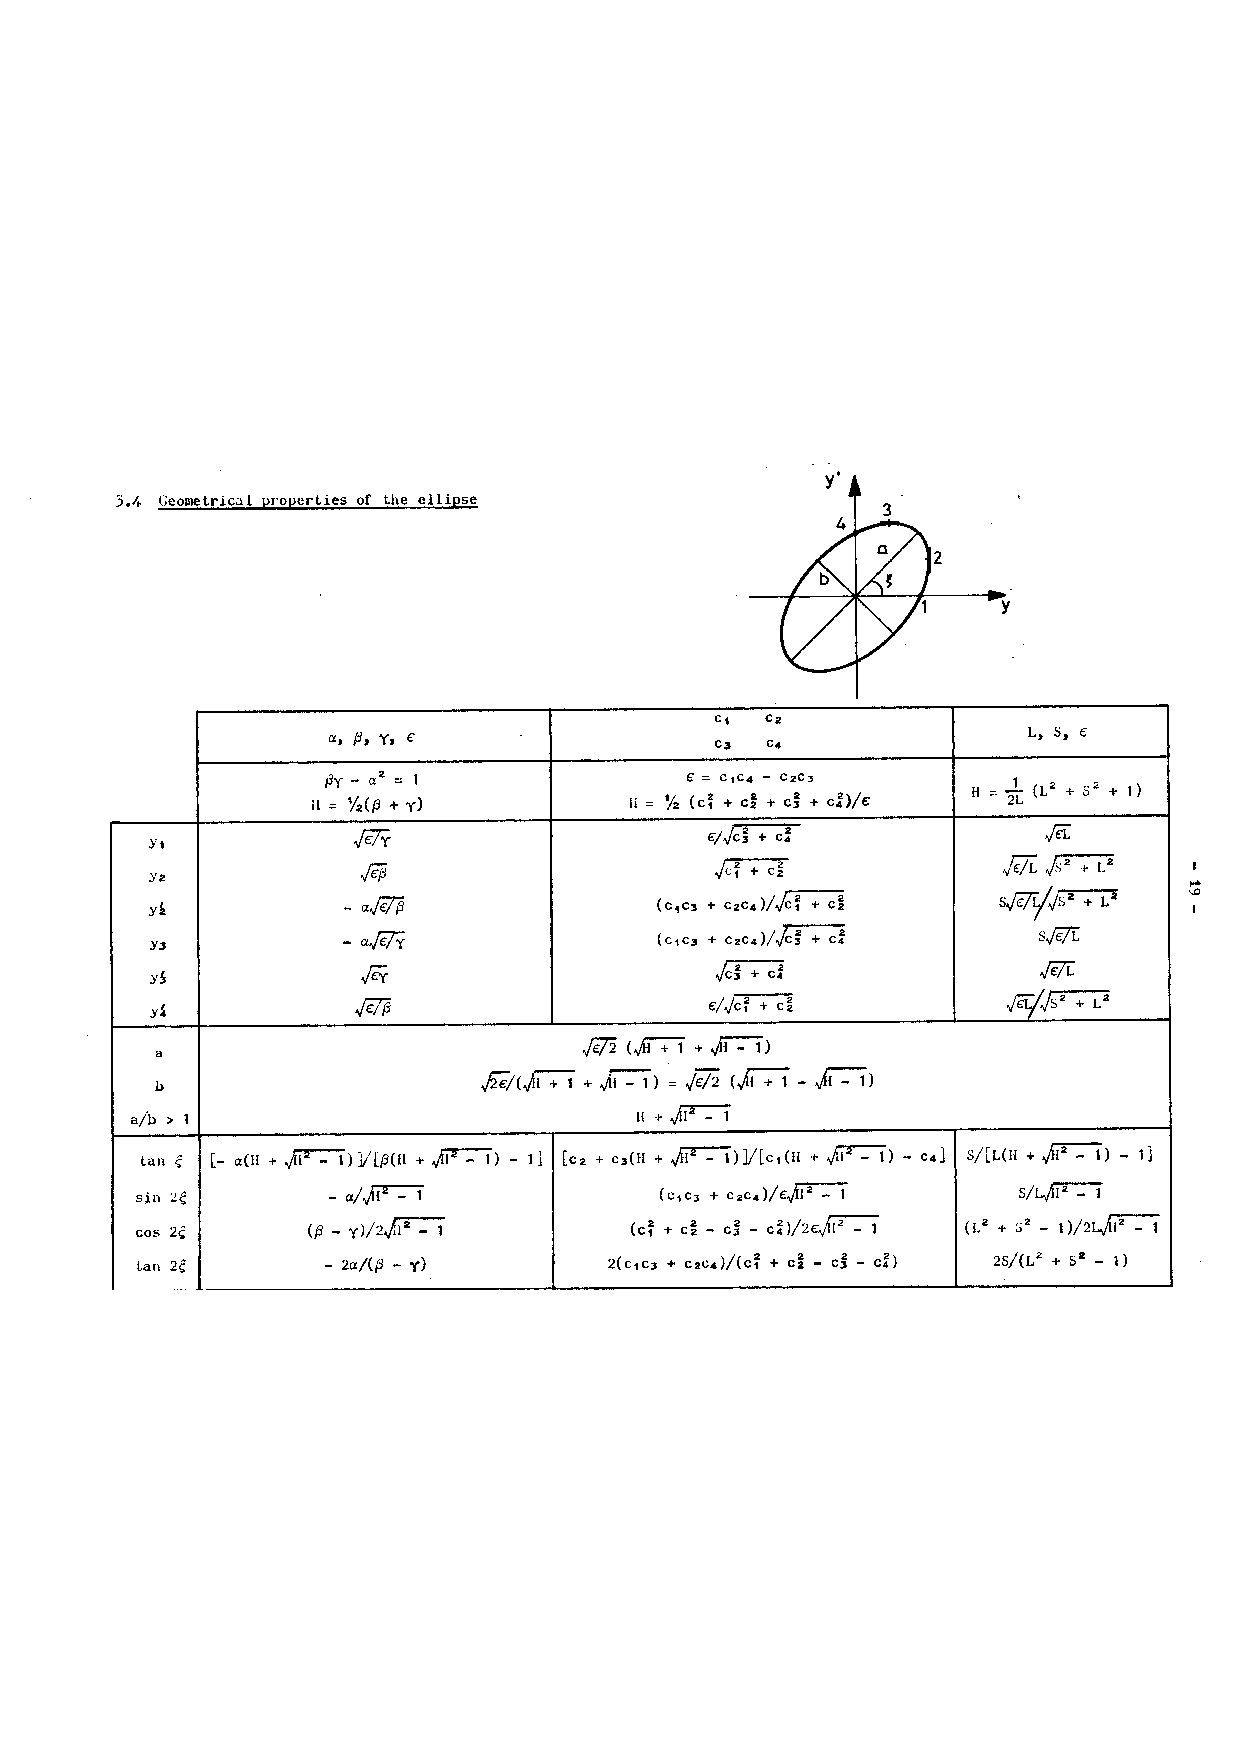
\includegraphics[width=15cm, trim={0.cm 7.6cm 0.cm 8.cm}, clip]{ellipse.pdf}
%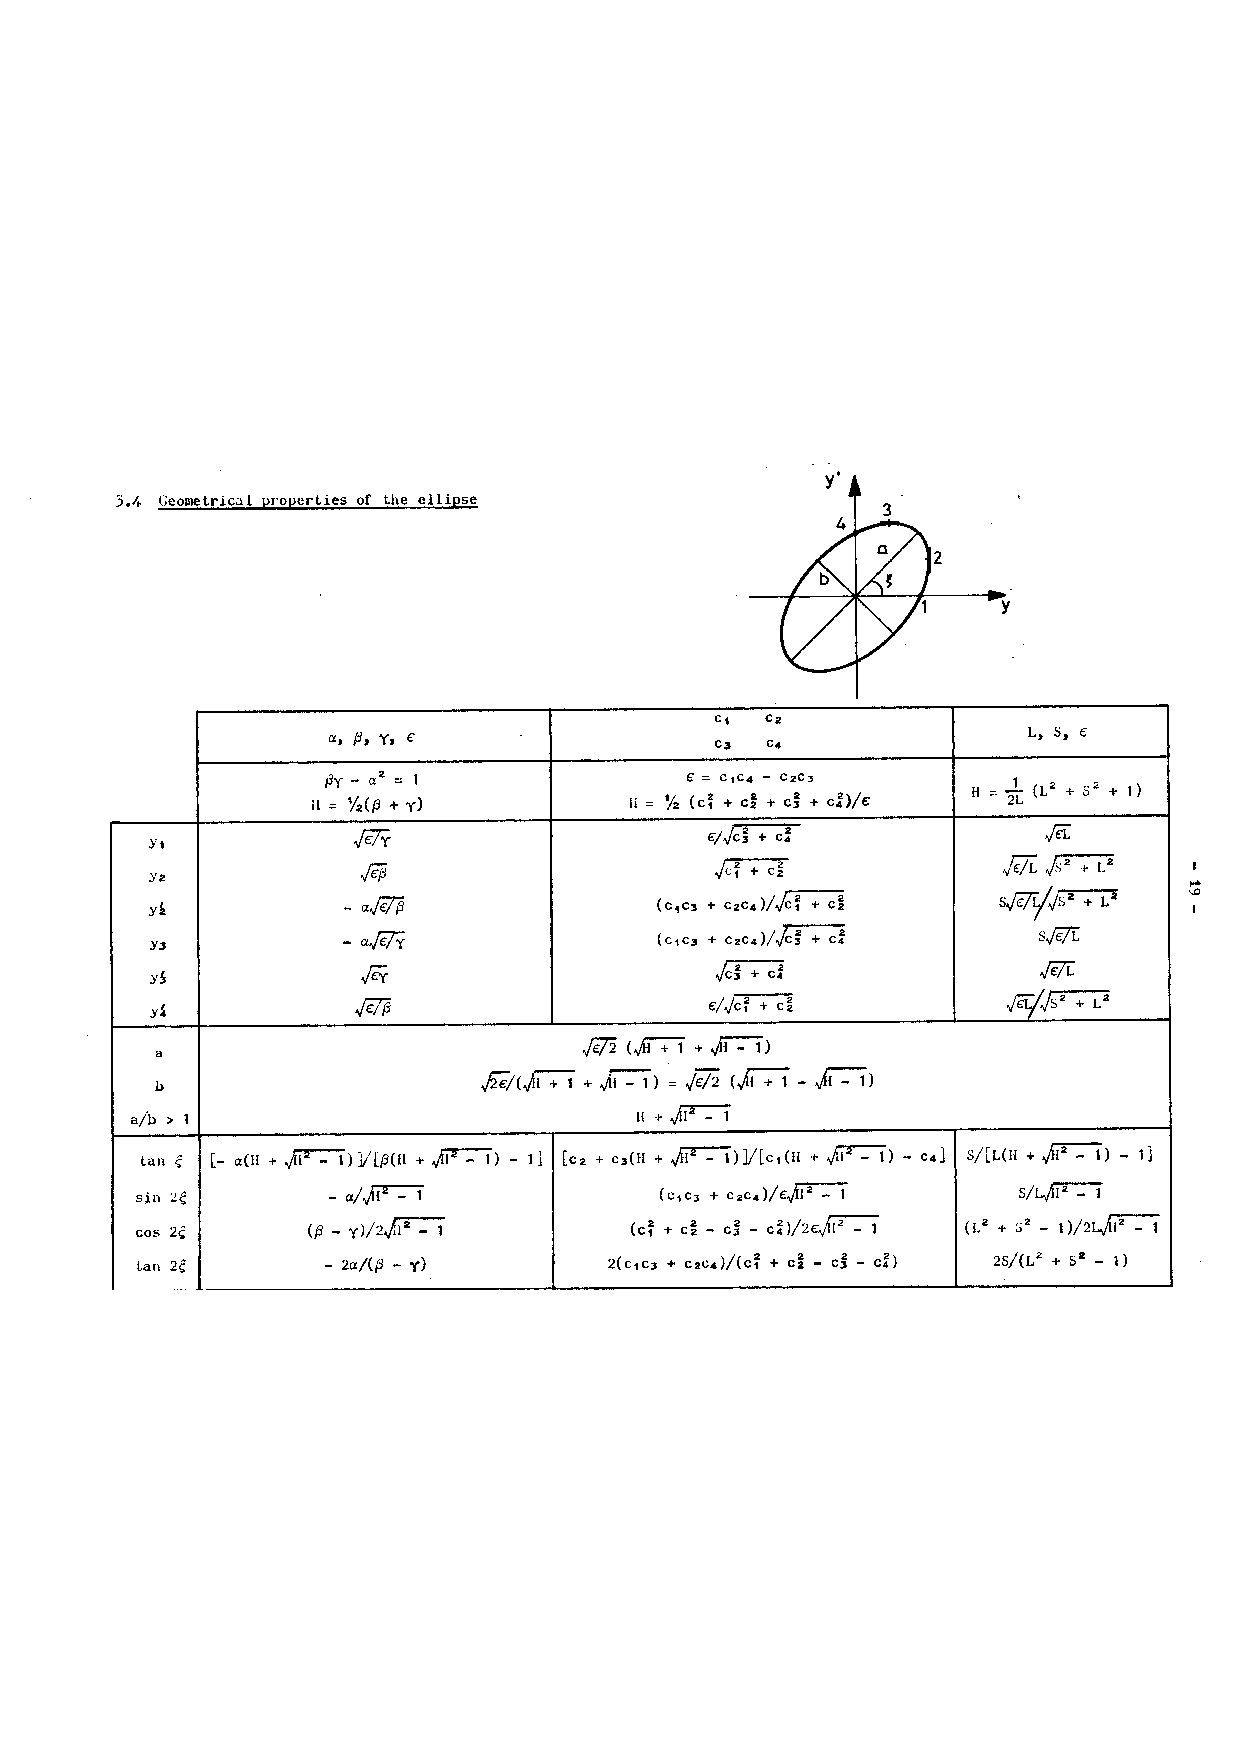
\includegraphics[width=1.4\textwidth}, clip]{ellipse.pdf}

\end{document}
